\section{Arquitetura do Sistema}
\label{sec:4.1}

O IGRIS adota um Monolito Modular com Adaptadores de Microsserviços, combinando a organização interna por módulos de domínio com o desacoplamento externo de componentes computacionalmente intensivos. O núcleo da aplicação é um único processo Spring Boot organizado em módulos coesos acadêmico, usuário, instituição, grade, segurança e comum, que se comunicam internamente sem latência de rede. Para a execução do Algoritmo Genético, o sistema delega o processamento a microsserviços independentes via adaptadores HTTP, isolando a lógica pesada de otimização sem comprometer a responsividade da API principal \cite[p.~15--16]{newman2021}.

A comunicação entre o Backend Core e os microsserviços ocorre de forma síncrona: o backend monta um \textit{payload} JSON com disponibilidades, matrizes, turmas e parâmetros do algoritmo, envia por HTTP POST ao microsserviço selecionado e recebe uma resposta estruturada contendo a grade otimizada, métricas de execução e lista de conflitos. Os parâmetros do algoritmo são armazenados na tabela \texttt{config\_sistema} e carregados em cache, permitindo ajuste em tempo de execução sem reinicialização \cite[p.~3]{newman2021}.

A arquitetura é composta por quatro serviços principais:

\begin{itemize}
  \item \textbf{Igris (Backend Core):} API principal em Java 17 com Spring Boot 3.5. Gerencia todas as operações CRUD do domínio acadêmico, autenticação JWT, controle de acesso RBAC e orquestra as chamadas aos microsserviços de otimização. É o único componente com acesso direto ao banco de dados PostgreSQL 15.
  \item \textbf{Sunny:} Microsserviço de geração de grade em Java com Spring Boot, implementando o Algoritmo Genético no paradigma orientado a objetos.
  \item \textbf{Morpheus:} Microsserviço equivalente em Python com Flask, implementando o mesmo algoritmo no paradigma funcional, com parada antecipada e melhoria local explícita.
  \item \textbf{Rocket:} Microsserviço em Go, implementando o AG com modelo de concorrência baseado em \textit{goroutines} e \textit{channels} (CSP). Representa o paradigma concorrente no benchmark comparativo \cite{coxbuday2017}.
\end{itemize}

Todos os componentes são containerizados via Docker e se comunicam pela rede interna \texttt{igris-network}, sem exposição direta ao exterior. O frontend React acessa exclusivamente o Backend Core na porta 8080 \cite[p.~20]{newman2021}.

\begin{figure}[H]
\centering
\caption{Arquitetura do sistema IGRIS}
\label{fig:arquitetura}

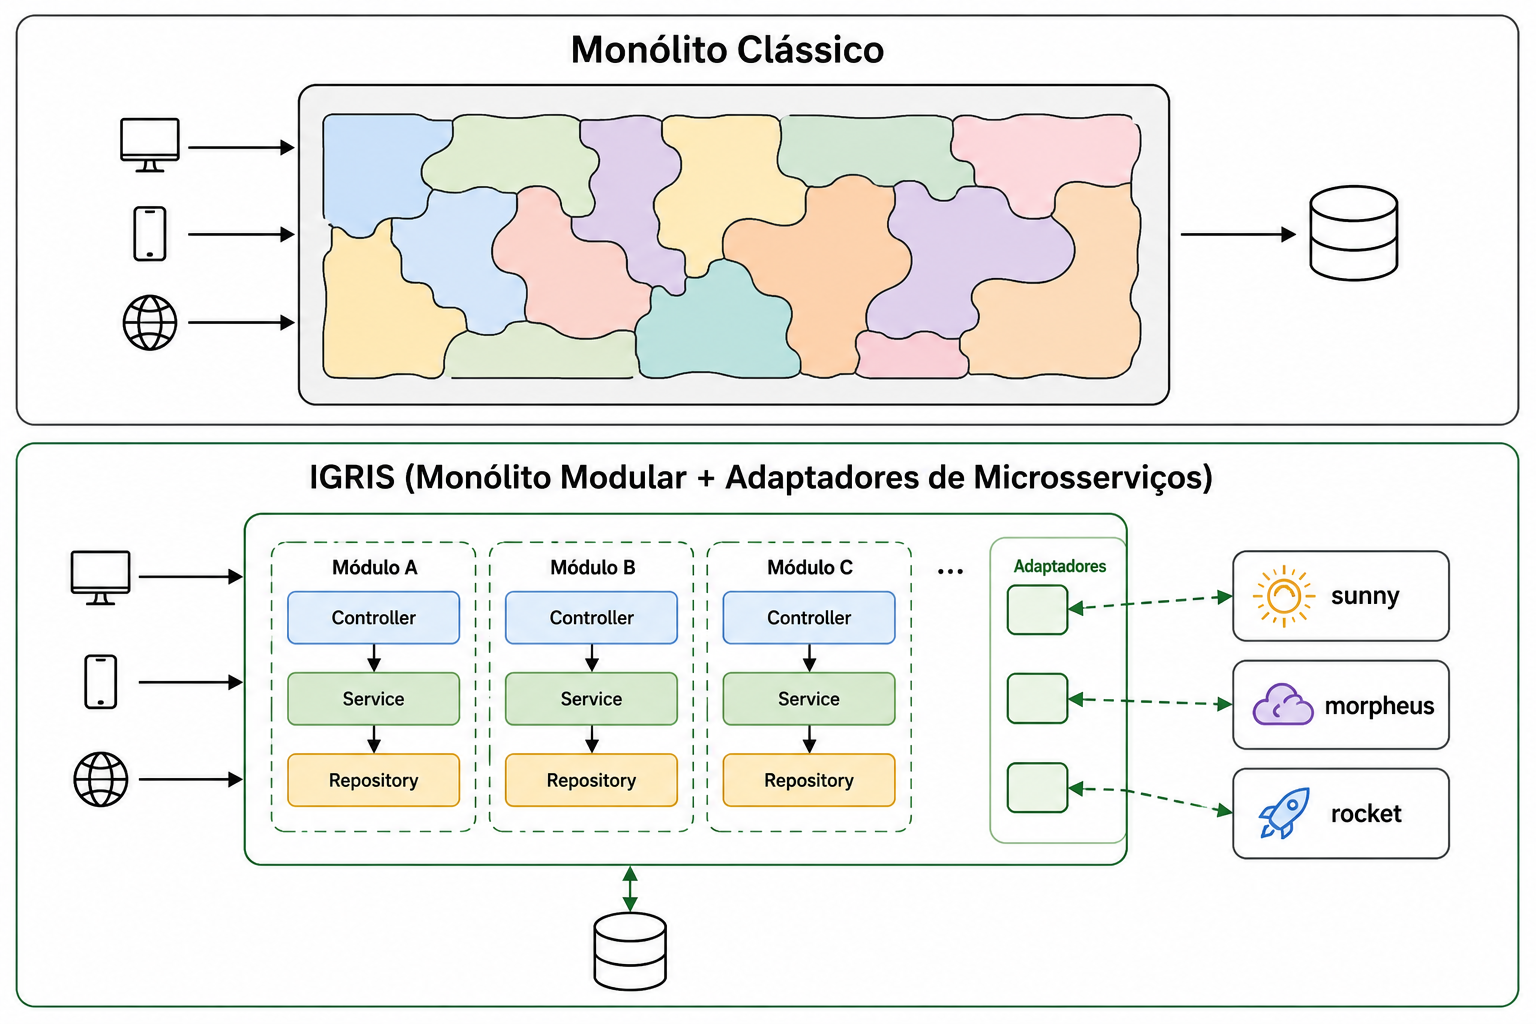
\includegraphics[width=0.85\textwidth]{figuras/Figura_8_ilustracaoArquitetura.png}

\vspace{0.2cm}
\fonteautores
\end{figure}